\chapter{FTP and TFTP}\label{ftp-and-tftp}

\section{The Purpose of FTP / TFTP}\label{the-purpose-of-ftp-tftp}

\begin{itemize}
\tightlist
\item
  FTP (File Transfer Protocol) and TFTP (Trivial File Transfer Protocol)
  are INDUSTRY STANDARD PROTOCOLS used to TRANSFER FILES over a NETWORK
\item
  They BOTH use a CLIENT-SERVER model

  \begin{itemize}
  \tightlist
  \item
    CLIENTS can use FTP / TFTP to COPY files FROM a SERVER
  \item
    CLIENTS can use FTP / TFTP to COPY files TO a SERVER
  \end{itemize}
\item
  As a NETWORK ENGINEER, the most common use for FTP / TFTP is in the
  process of UPGRADING the OPERATING SYSTEM of a NETWORK DEVICE
\item
  You can use FTP / TFTP to DOWNLOAD the newer version of IOS from a
  SERVER and then REBOOT the DEVICE with the new IOS image
\end{itemize}

\begin{figure}
\centering
\pandocbounded{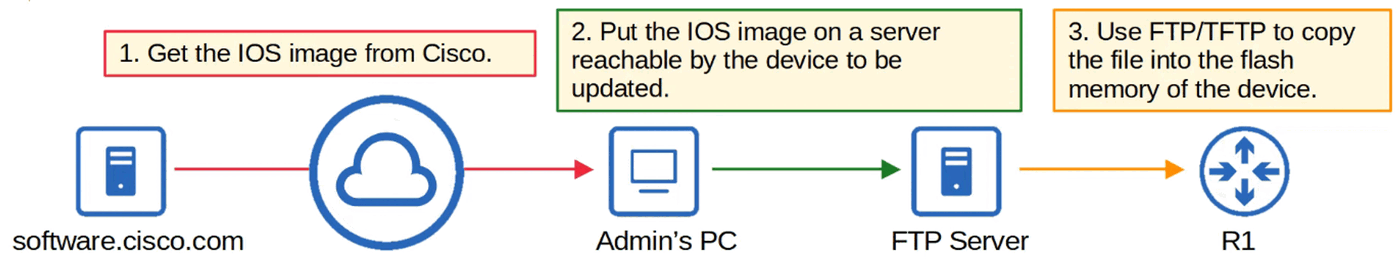
\includegraphics[keepaspectratio,alt={image}]{images/44-ftp-and-tftp/img-001.png}}
\end{figure}

TFTP and FTP FUNCTIONS AND DIFFERENCES

\section{TFTP}\label{tftp}

\begin{itemize}
\tightlist
\item
  TFTP first standardized in 1981
\item
  Named ``Trivial'' because it's SIMPLE and has only basic features
  compared to FTP

  \begin{itemize}
  \tightlist
  \item
    Only allows a CLIENT to COPY FILES to / from a SERVER
  \end{itemize}
\item
  Was released after FTP, but not a REPLACEMENT for FTP.

  \begin{itemize}
  \tightlist
  \item
    It's another tool to use when LIGHTWEIGHT SIMPLICITY is more
    important than FUNCTIONALITY
  \end{itemize}
\item
  NO AUTHENTICATION (Username / Password) so SERVERS will respond to ALL
  FTP REQUESTS
\item
  NO ENCRYPTION. All DATA is sent PLAIN TEXT
\item
  Best used in a CONTROLLED environment to transfer SMALL FILES quickly
\item
  TFTP SERVERS listen on UDP PORT 69
\item
  UDP is CONNECTIONLESS and doesn't provided RELIABILITY with
  RETRANSMISSIONS
\item
  However, TFTP has SIMILAR built-in FEATURES within the PROTOCOL itself
\end{itemize}

\section{TFTP Reliability}\label{tftp-reliability}

\begin{itemize}
\tightlist
\item
  Every TFTP DATA message is ACKNOWLEDGED

  \begin{itemize}
  \tightlist
  \item
    If the CLIENT is transferring a FILE TO the SERVER, the SERVER will
    send ACK messages
  \item
    If the SERVER is transferring a FILE TO the CLIENT, the CLIENT will
    send ACK messages
  \end{itemize}
\item
  TIMERS are used, and if an EXPECTED message isn't received in time,
  the waiting DEVICE will RESEND its previous message.
\end{itemize}

\begin{figure}
\centering
\pandocbounded{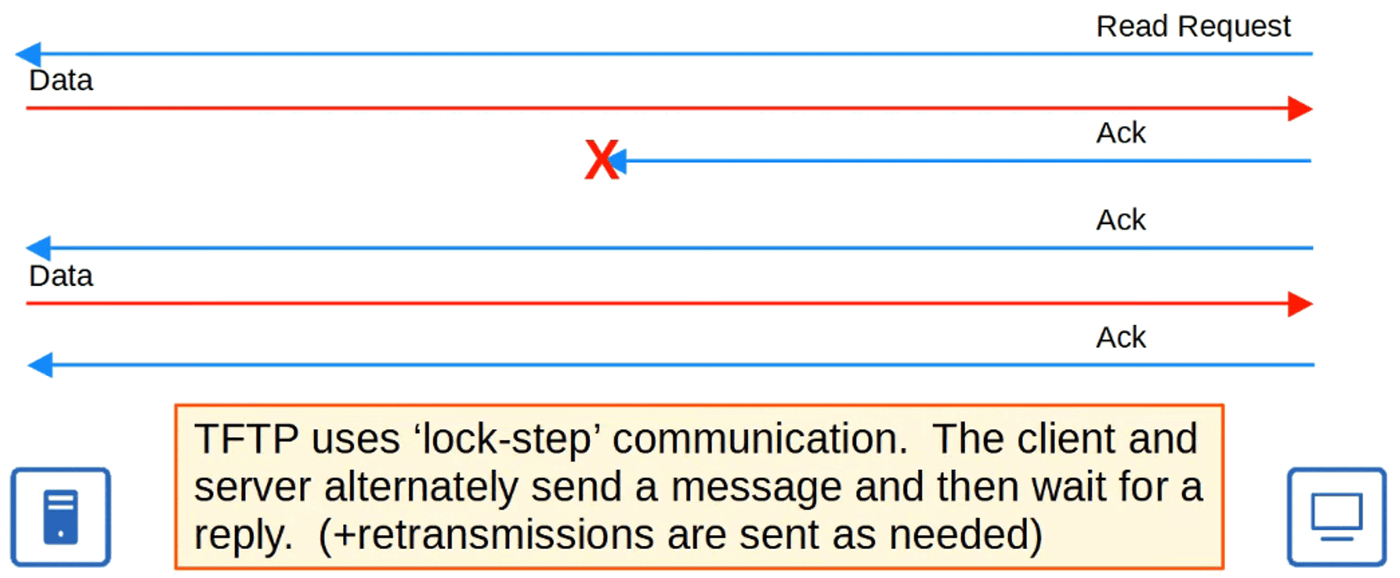
\includegraphics[keepaspectratio,alt={image}]{images/44-ftp-and-tftp/img-002.png}}
\end{figure}

TFTP ``CONNECTIONS''

\begin{figure}
\centering
\pandocbounded{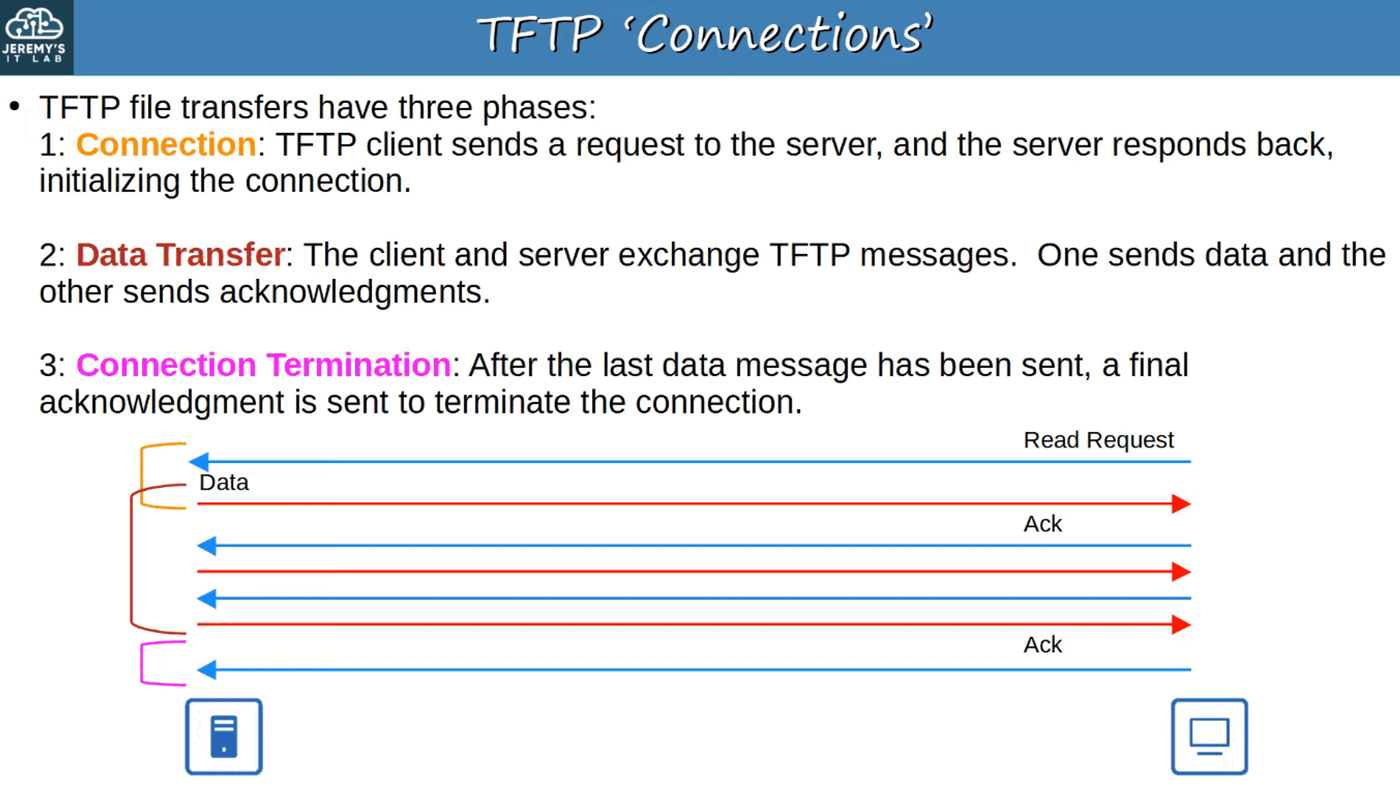
\includegraphics[keepaspectratio,alt={image}]{images/44-ftp-and-tftp/img-003.png}}
\end{figure}

TFTP TID (Not in the CCNA exam)

\begin{itemize}
\tightlist
\item
  When the CLIENT sends the FIRST message to the SERVER, the DESTINATION
  PORT is UDP 69 and the SOURCE PORT is a random EPHEMERAL PORT
\item
  This ``random port'' is called a ``TRANSFER IDENTIFIER'' (TID) and
  identifies the DATA TRANSFER
\item
  The SERVER then also selects a RANDOM TID to use as a SOURCE PORT when
  it replies, NOT UDP 69
\item
  When the CLIENT sends the NEXT message, the DESTINATION PORT will be
  the SERVER'S TID, NOT UDP 69
\end{itemize}

UDP PORT 69 (TFTP) is only used at the initial request message

\begin{figure}
\centering
\pandocbounded{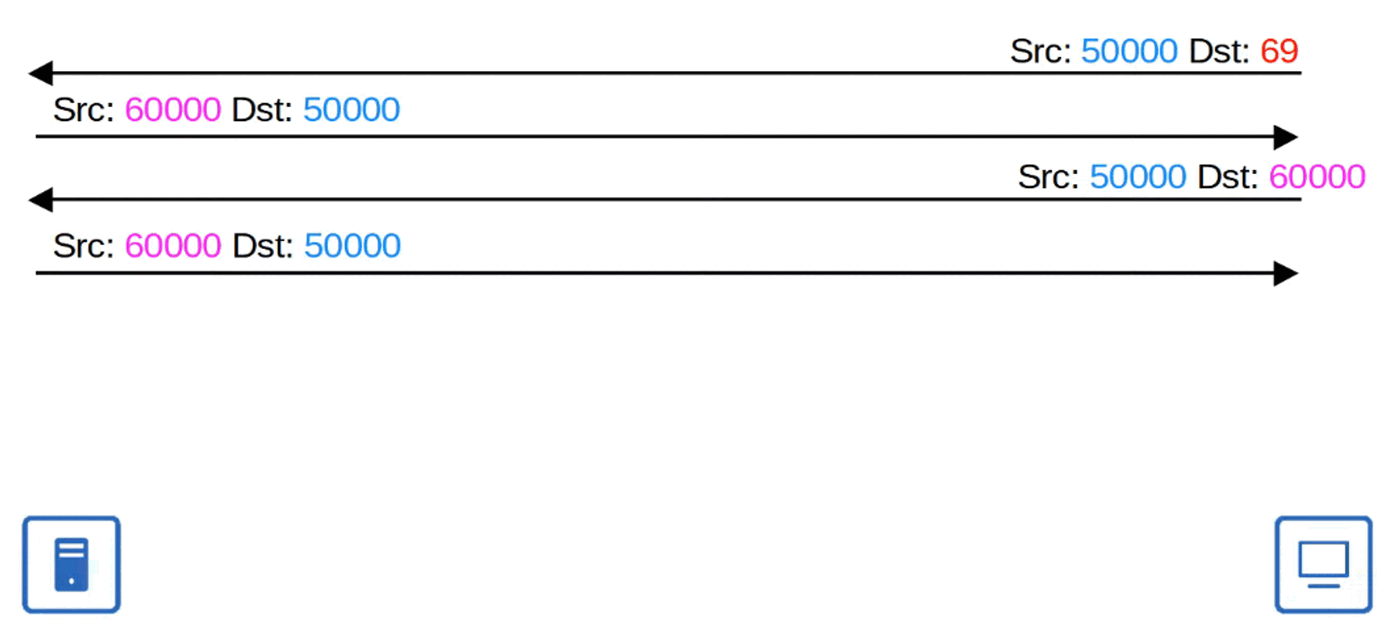
\includegraphics[keepaspectratio,alt={image}]{images/44-ftp-and-tftp/img-004.png}}
\end{figure}

\section{FTP}\label{ftp}

\begin{itemize}
\tightlist
\item
  FTP was first standardized in 1971
\item
  FTP uses TCP PORTS 20 and 21
\item
  USERNAMES and PASSWORDS are used for AUTHENTICATION, however there is
  NO ENCRYPTION
\item
  For GREATER security, FTPS (FTP over SSL / TLS) can be used (Upgrade
  to FTP)
\item
  SSH File Transfer Protocol (SFTP) can also be used for GREATER
  security (New Protocol)
\item
  FTP is MORE complex than TFTP and ALLOWS not only FILE TRANSFERS but
  CLIENTS can also:

  \begin{itemize}
  \tightlist
  \item
    Navigate FILE DIRECTORIES
  \item
    ADD / REMOVE FILES
  \item
    LIST FILES
  \item
    etc\ldots{}
  \end{itemize}
\item
  The CLIENT sends FTP \emph{commands} to the SERVER to perform these
  functions
\end{itemize}

\section{FTP Control Connections}\label{ftp-control-connections}

\begin{itemize}
\tightlist
\item
  FTP uses TWO TYPES of connections:

  \begin{itemize}
  \tightlist
  \item
    An FTP CONTROL connection (TCP 21) is established and used to send
    FTP commands and replies
  \item
    When FILES or DATA are to be transferred, separate FTP DATA (TCP 20)
    connections are established and terminated as needed
  \end{itemize}
\end{itemize}

\begin{figure}
\centering
\pandocbounded{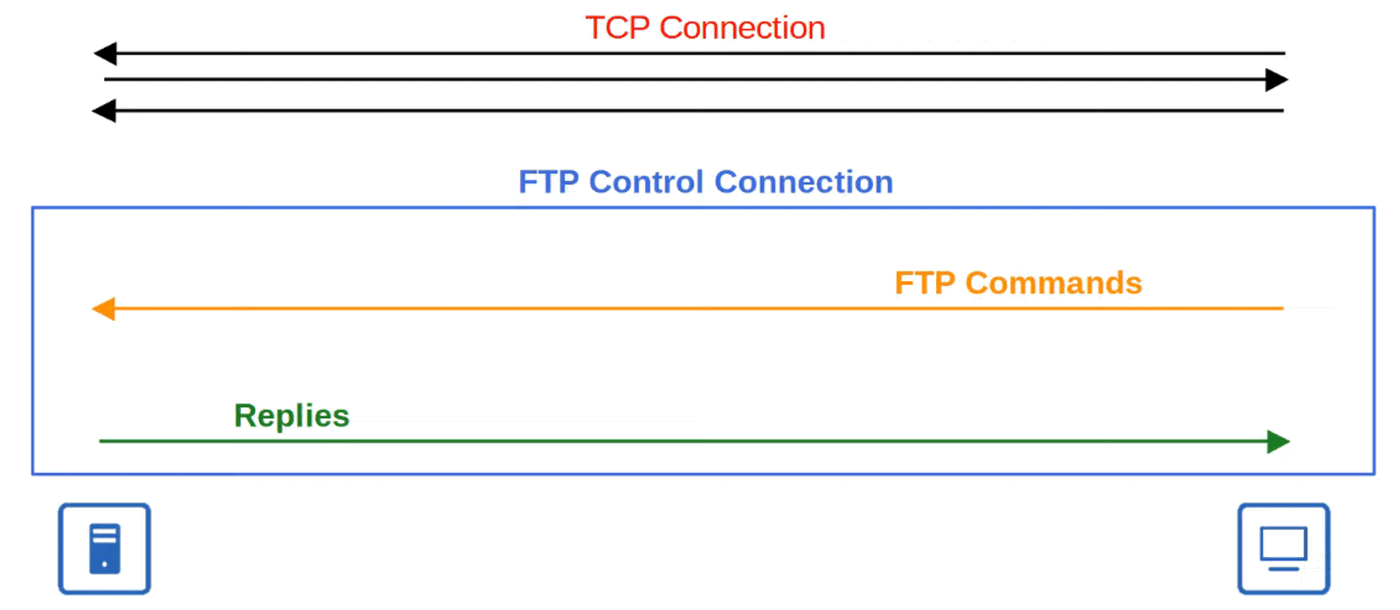
\includegraphics[keepaspectratio,alt={image}]{images/44-ftp-and-tftp/img-005.png}}
\end{figure}

\section{Active Mode FTP Data
Connections}\label{active-mode-ftp-data-connections}

\begin{itemize}
\tightlist
\item
  The DEFAULT method of establishing FTP DATA connections is ACTIVE MODE
  in which the SERVER initiates the TCP connection.
\end{itemize}

\begin{figure}
\centering
\pandocbounded{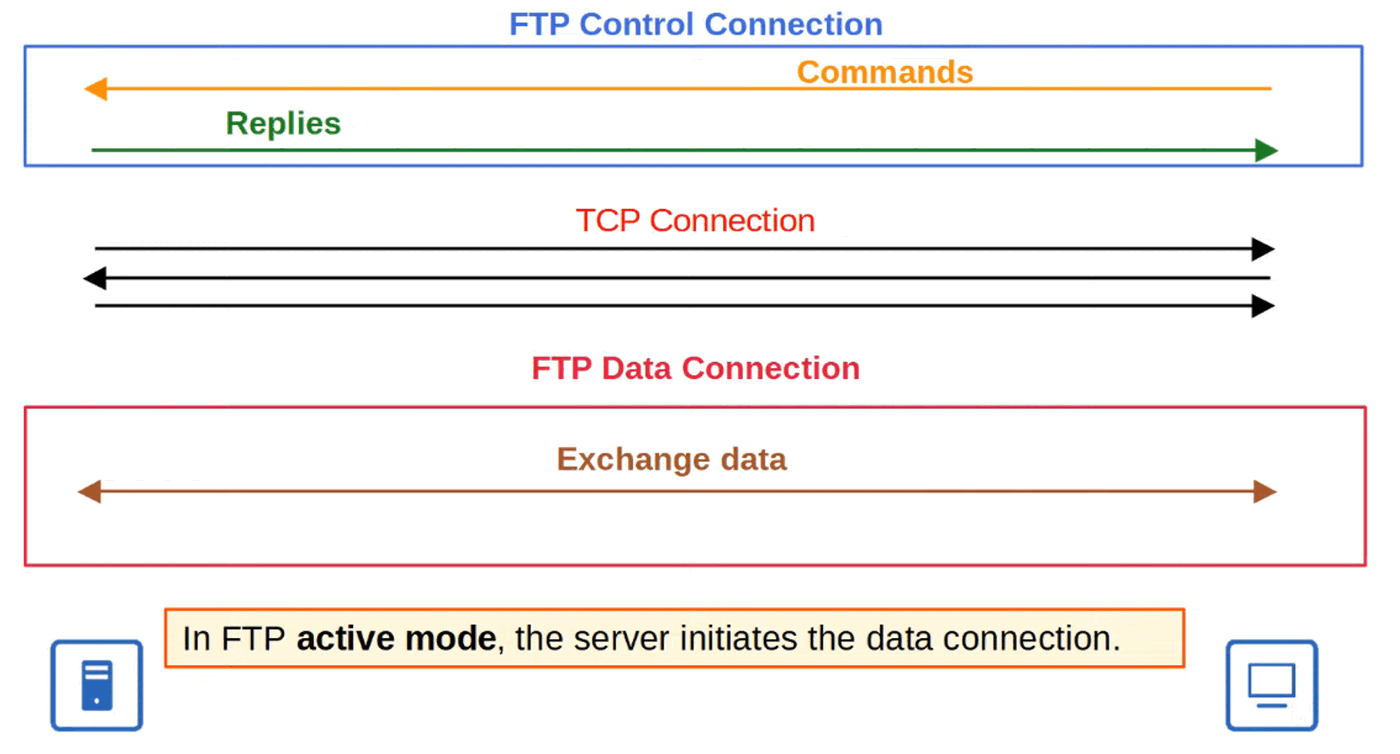
\includegraphics[keepaspectratio,alt={image}]{images/44-ftp-and-tftp/img-006.png}}
\end{figure}

\begin{itemize}
\tightlist
\item
  In FTP PASSIVE MODE, the CLIENT initiates the DATA connection.

  \begin{itemize}
  \tightlist
  \item
    This is often necessary when the CLIENT is behind a FIREWALL, which
    could BLOCK the INCOMING CONNECTION from the SERVER
  \end{itemize}
\end{itemize}

\begin{figure}
\centering
\pandocbounded{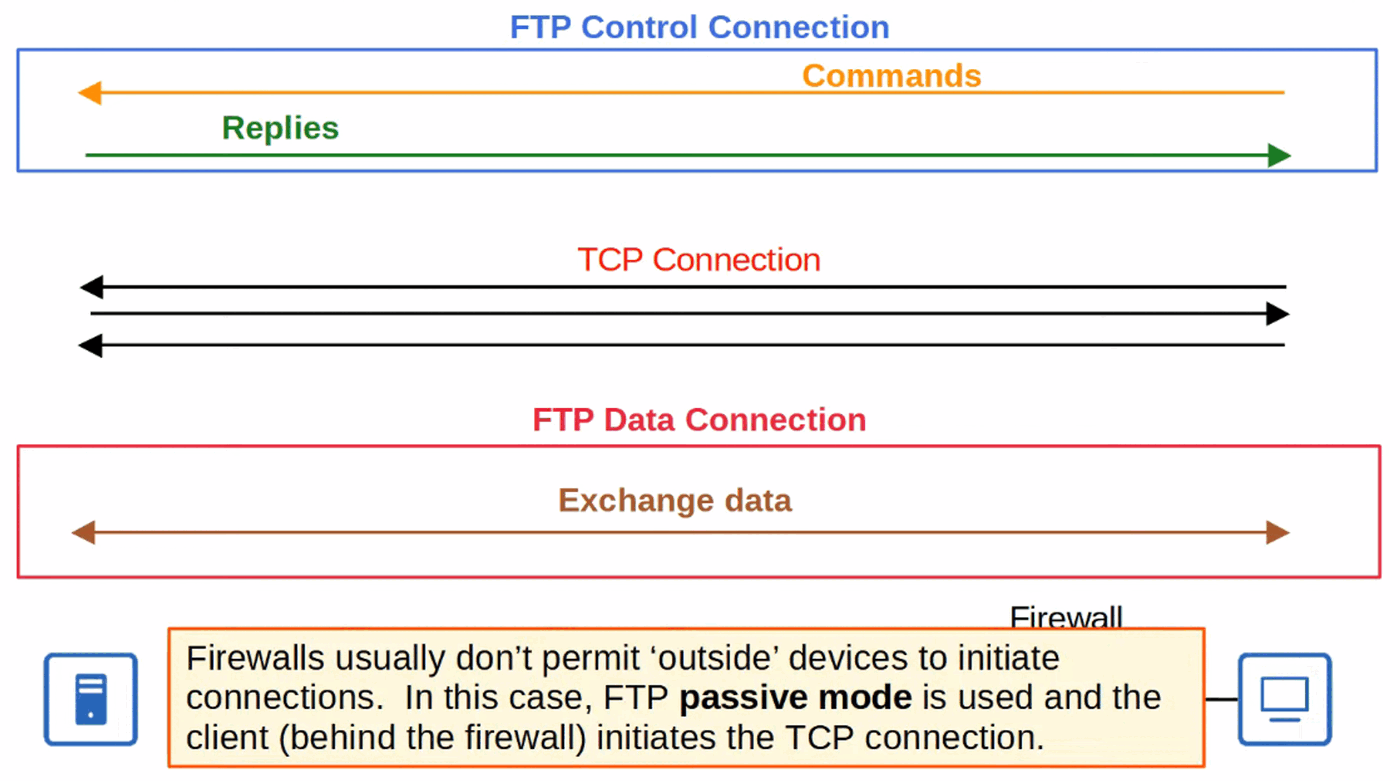
\includegraphics[keepaspectratio,alt={image}]{images/44-ftp-and-tftp/img-007.png}}
\end{figure}

\section{FTP Versus TFTP}\label{ftp-versus-tftp}

\begin{figure}
\centering
\pandocbounded{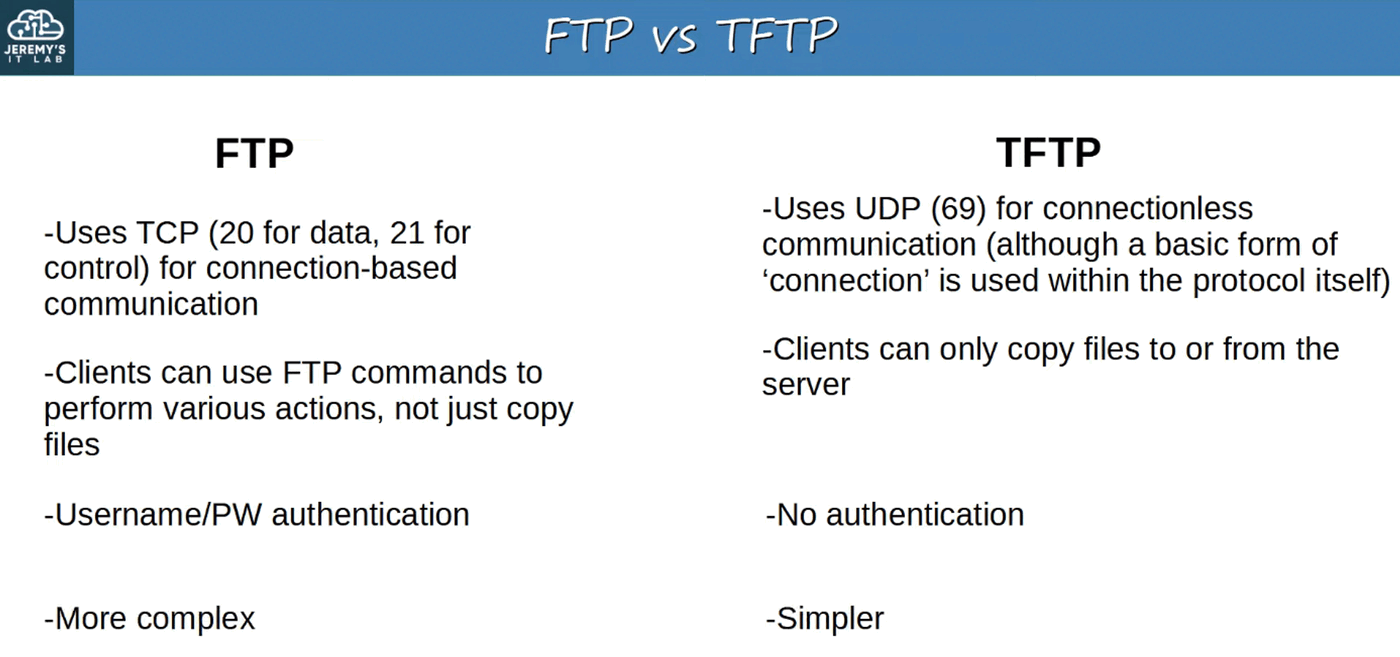
\includegraphics[keepaspectratio,alt={image}]{images/44-ftp-and-tftp/img-008.png}}
\end{figure}

\section{IOS File Systems}\label{ios-file-systems}

\begin{itemize}
\tightlist
\item
  A FILE SYSTEM is a way of controlling how DATA is STORED and RETRIEVED
\item
  You can VIEW the FILE SYSTEM of a Cisco IOS DEVICE with
  \passthrough{\lstinline!show file systems!}
\end{itemize}

\begin{figure}
\centering
\pandocbounded{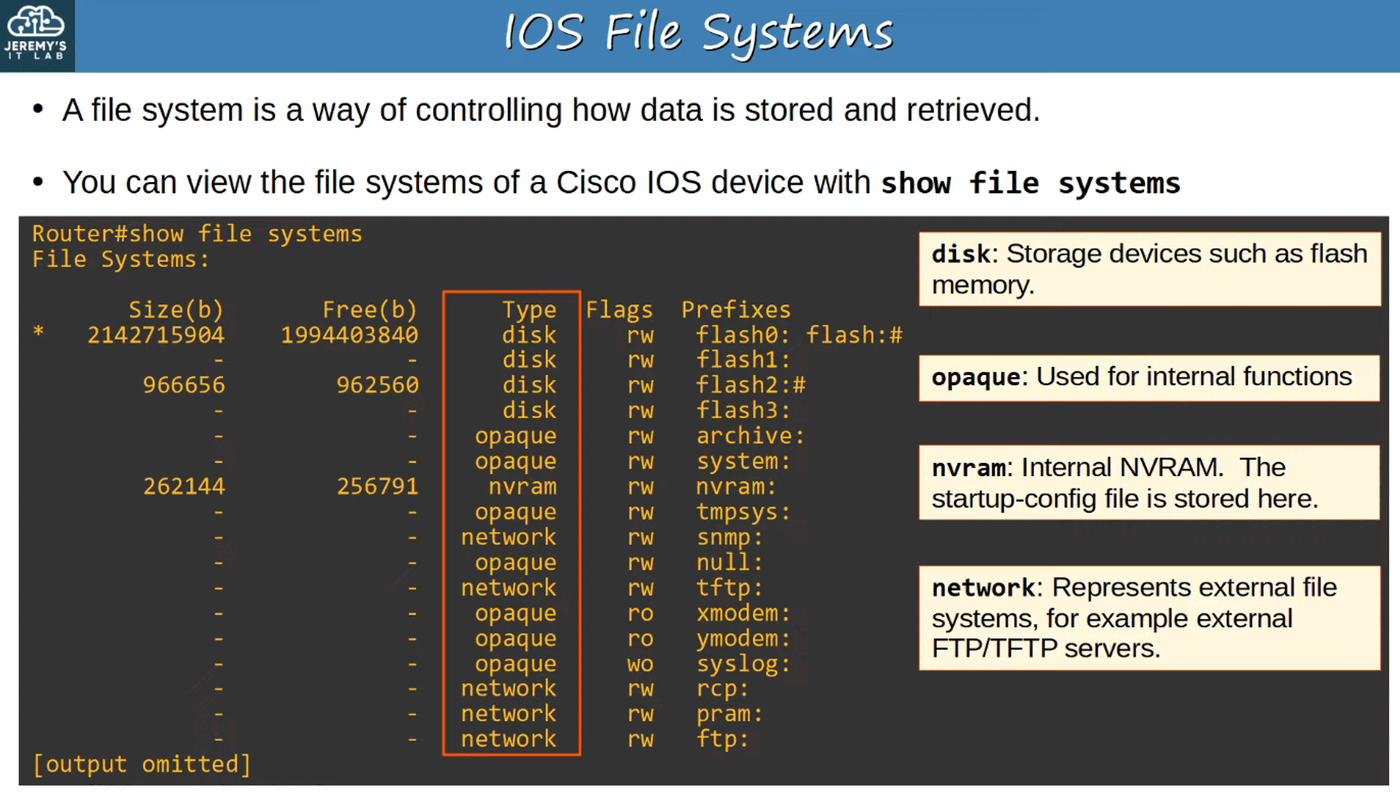
\includegraphics[keepaspectratio,alt={image}]{images/44-ftp-and-tftp/img-009.png}}
\end{figure}

\section{Using FTP / TFTP in IOS}\label{using-ftp-tftp-in-ios}

\begin{itemize}
\tightlist
\item
  You can VIEW the current version of IOS with
  \passthrough{\lstinline!show version!}
\end{itemize}

\begin{figure}
\centering
\pandocbounded{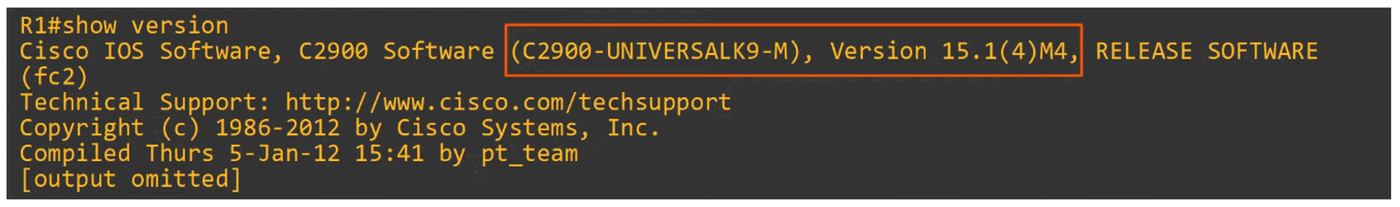
\includegraphics[keepaspectratio,alt={image}]{images/44-ftp-and-tftp/img-010.png}}
\end{figure}

\begin{itemize}
\tightlist
\item
  You can VIEW the contents of flash with
  \passthrough{\lstinline!show flash!}
\end{itemize}

\begin{figure}
\centering
\pandocbounded{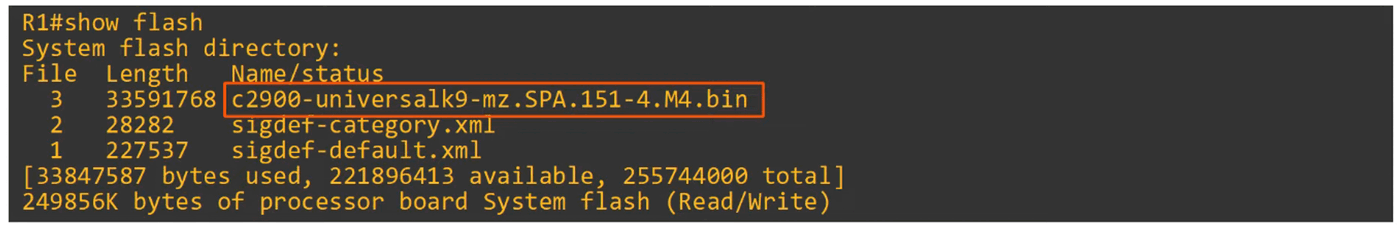
\includegraphics[keepaspectratio,alt={image}]{images/44-ftp-and-tftp/img-011.png}}
\end{figure}

\section{Copying Files with TFTP}\label{copying-files-with-tftp}

\section{Step 1}\label{step-1}

\begin{figure}
\centering
\pandocbounded{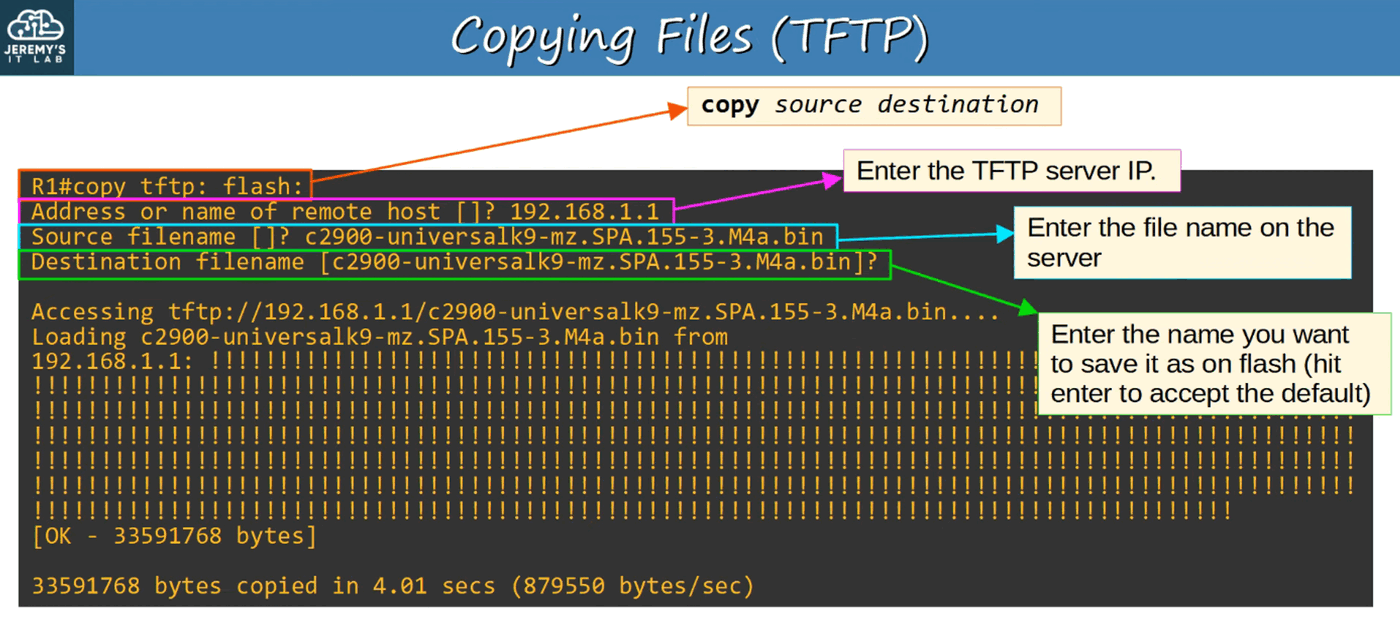
\includegraphics[keepaspectratio,alt={image}]{images/44-ftp-and-tftp/img-012.png}}
\end{figure}

\section{Step 2}\label{step-2}

\begin{figure}
\centering
\pandocbounded{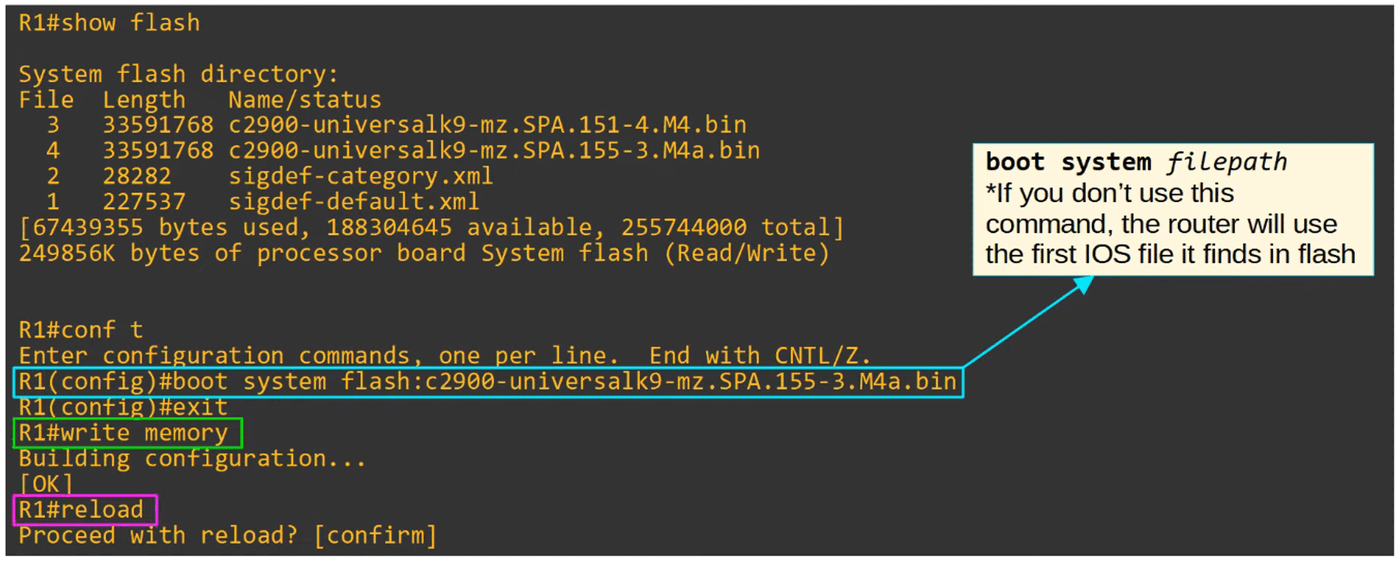
\includegraphics[keepaspectratio,alt={image}]{images/44-ftp-and-tftp/img-013.png}}
\end{figure}

\section{Step 3}\label{step-3}

\begin{figure}
\centering
\pandocbounded{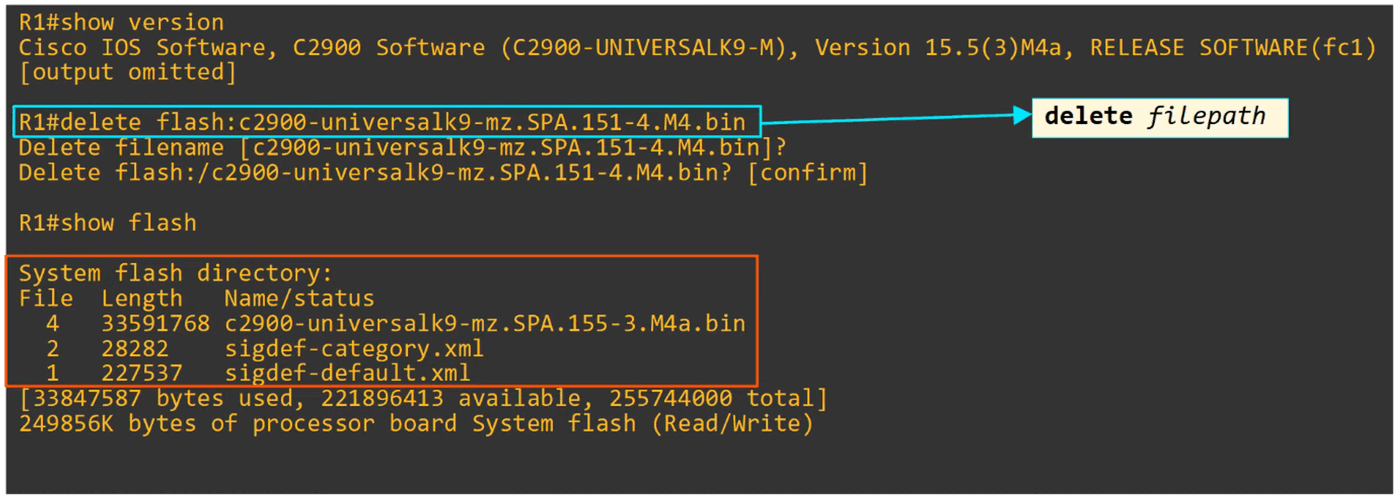
\includegraphics[keepaspectratio,alt={image}]{images/44-ftp-and-tftp/img-014.png}}
\end{figure}

\section{Copying Files with FTP}\label{copying-files-with-ftp}

\section{Step 1}\label{step-1-1}

\begin{figure}
\centering
\pandocbounded{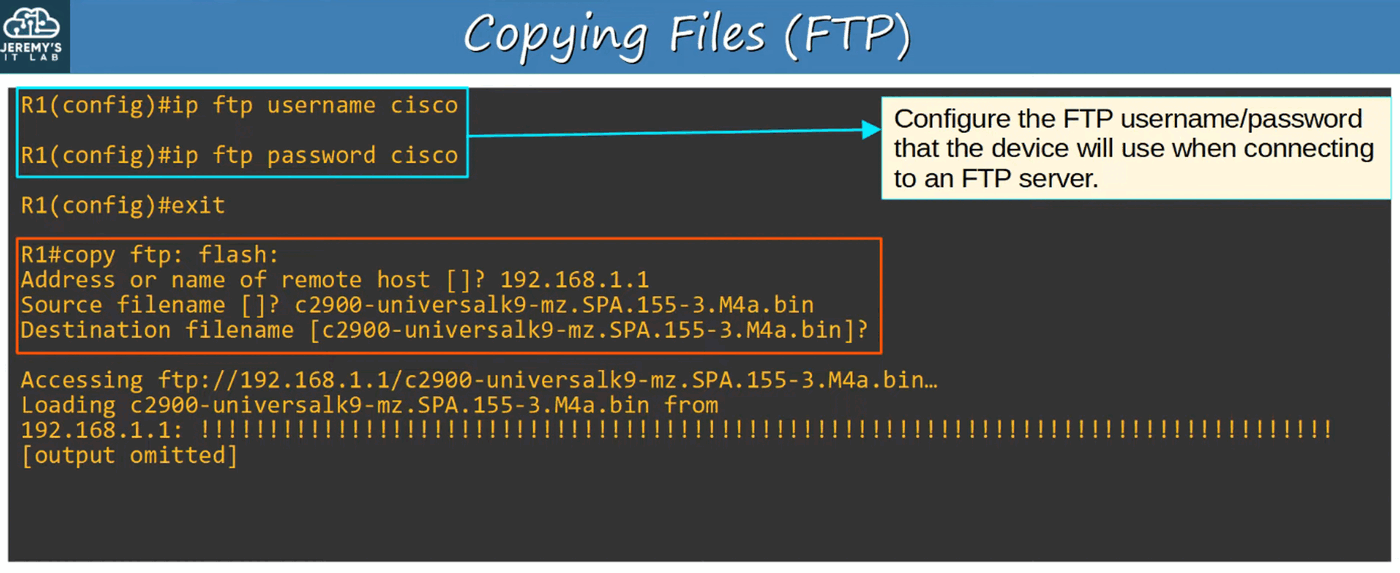
\includegraphics[keepaspectratio,alt={image}]{images/44-ftp-and-tftp/img-015.png}}
\end{figure}

STEP 2 and 3 identical to TFTP above

\section{Command Summary}\label{command-summary}

\begin{figure}
\centering
\pandocbounded{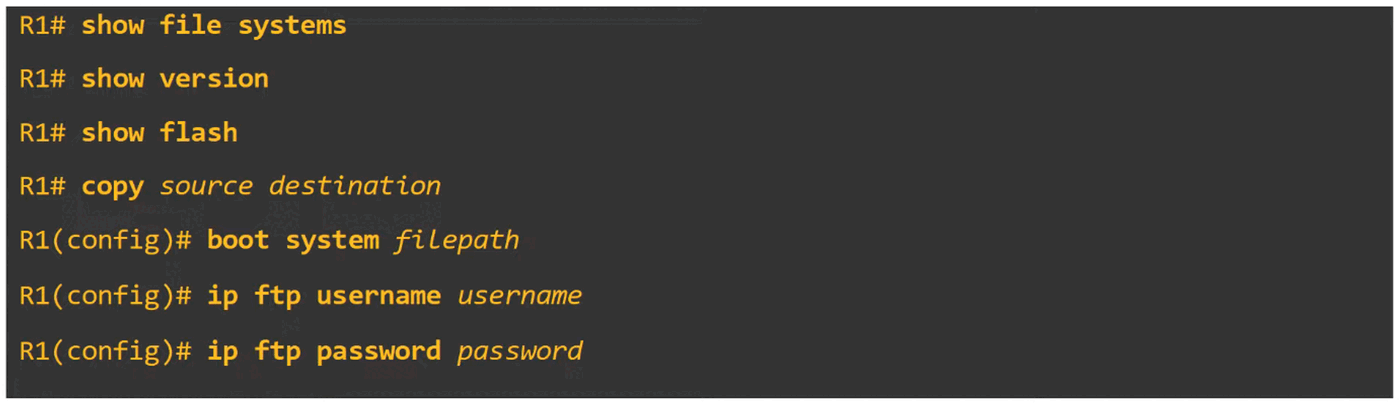
\includegraphics[keepaspectratio,alt={image}]{images/44-ftp-and-tftp/img-016.png}}
\end{figure}
